
\chapter{Show}
\minitoc 


\section{General options.} 
\begin{figure}
  \centering
  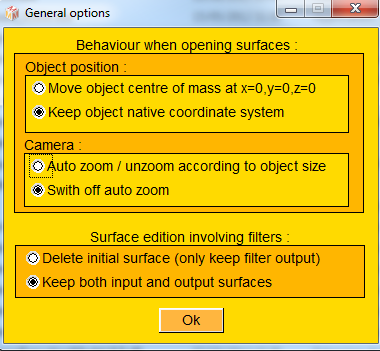
\includegraphics[scale=0.5]{images/Show/General_options_window.png} 
	\caption{General options window.}
\label{general_options_window}
 
\end{figure}


The general options window (see Fig. \ref{general_options_window}) contains the following sections:
\subsection{Behaviour when opening surface}
\textbf{\underline{Object position:}}\\
- \textit{Move object centre of mass at x=0, y=0, z=0}: when active,
the position matrix of a newly opened surface is set in
order to display the object at the origin of the coordinate
system (x=0, y=0, z=0). This option is useful when surface
native coordinate system is far from the origin (this is often
the case if you see nothing in the 3D rendering window
after opening a surface).\\
- \textit{Keep object native coordinate system}: when active, the
position matrix of a newly opened surface is set to the identity matrix.\\\\
\noindent
\textbf{\underline{Camera:}}\\
- \textit{Auto zoom / unzoom according to object size}: when active, the zoom of the camera is modified in
order to match the object global size.\\
- Switch off auto zoom: switches off the preceding option.
 
\subsection{Surface edition involving filters}
The following ``filters" are available in ISE-MeshTools (see ``Edit selected surfaces" section):\\
- Connectivity filters\\
- Lasso cut\\
- TPS deformation\\
- Mesh mirroring/smoothing/decimation/densification/hole filling\\\\
\noindent
\textbf{\underline{Delete initial surface (only keep filter output)}}: when active, when using one of the previously
mentioned filters, the initial object is deleted. Only the filter output is kept. This option is useful to
avoid object multiplication.\\\\
\noindent
\textbf{\underline{Keep both input and output surfaces}}: when active, when using one of the previously mentioned
filters, the initial object is kept. This option is useful to compare the initial object and the filter output.\\
Note that filter output object’s name differs from filter input objects’ name.

\section{Show object view/hide window.}
This window (see Fig. \ref{view_hide_objects}) shows the list of currently opened meshes. You may hide / show objects using this interface. Note that if
you delete/load objects while opened, the list will not be updated. Please click on ``refresh" to see the actual current
list of existing objects.\\\\
``Check all" : will show all objects\\\\
``uncheck all" : will hide all currently loaded objects.\\\\
This window is useful to hide/show structures.

\begin{figure}
  \centering
  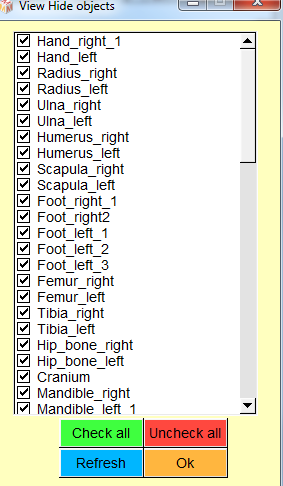
\includegraphics[scale=0.7]{images/Show/View_hide_objects_window.png} 
	\caption{View Hide Objects window.}
\label{view_hide_objects}
 
\end{figure}



\section{Area and volume of selected objects.}
This option shows in the output window the list of surface objects which are selected.

\section{Print scalar list.}
This option shows in the output window the list of existing scalars. When saving .vtk files, all these
scalars are saved inside the .vtk file along with the geomtry of the object(s). When saving .ply files,
only the RGB scalars are saved.

\section{Print list of selected objects.}
This option shows in the output window the full list of the names of all currently selected surfaces.
\section{Print list of distinct selected objects.}
This option shows in the output window the list of the distinct names of all currently selected
surfaces. It may sometimes be useful to compare the full list of names and the list of distinct names
of selected objects when working with projects : ISE-MeshTools only allows to save series of surface
files having distinct names (see tutorial ``Working with projects" for futher explanations).
\section{Show object display order.}
This option shows in the output window the list of objects (landmarks, target landmarks, flag landmarks, logical objects, surfaces) loaded into ISE-MeshTools, as well as their display order.